\documentclass[11pt]{article}
\usepackage[T1]{fontenc}
\usepackage[utf8]{inputenc}
\usepackage{lmodern,microtype}
\usepackage[a4paper,margin=25mm]{geometry}
\usepackage{amsmath,amssymb,amsthm,mathtools}
\usepackage{booktabs,array,tabularx,graphicx,xcolor,enumitem}
\usepackage{float}
\usepackage{fancyhdr}
\usepackage[colorlinks=true,linkcolor=blue!45!black,citecolor=blue!45!black,urlcolor=blue!45!black,breaklinks=true]{hyperref}
\usepackage{bookmark}
\definecolor{ink}{HTML}{18354A}
\definecolor{accent}{HTML}{146C94}
\newcommand{\F}{\mathbb F_q}
\newcommand{\Sp}{\operatorname{Sp}}
\newcommand{\TV}{d_{\mathrm{TV}}}
\newcommand{\Law}{\mathcal L}
\newcommand{\rank}{\operatorname{rank}}
\newcommand{\rad}{\operatorname{rad}}
\newcommand{\Mat}{\operatorname{Mat}}
\newcommand{\E}{\mathbb E}
\newcommand{\1}{\mathbf 1}
\newcommand{\gb}[2]{\genfrac{[}{]}{0pt}{}{#1}{#2}_{q}}
\newcommand{\bink}{\binom{k}{2}}
\newcommand{\src}[2]{\href{https://github.com/lsernau/grh-lean/blob/72fead102f663d5c7a407964a13dc0cf9d977207/#1}{#2}}
\newcommand{\prior}[2]{\href{https://github.com/VladimirReshetnikov/ProveIt/blob/9ce7302df13ca8ea547135be83c794141da8d79c/Analysis/GeneralizedRiemannHypothesis/#1}{#2}}
\newtheorem{theorem}{Theorem}[section]
\newtheorem{lemma}[theorem]{Lemma}
\newtheorem{proposition}[theorem]{Proposition}
\newtheorem{corollary}[theorem]{Corollary}
\theoremstyle{definition}
\newtheorem{definition}[theorem]{Definition}
\theoremstyle{remark}
\newtheorem{remark}[theorem]{Remark}
\numberwithin{equation}{section}
\setlist{itemsep=3pt,topsep=5pt}
\setlength{\parskip}{3pt}
\setlength{\headheight}{14pt}
\pagestyle{fancy}
\fancyhf{}
\fancyhead[L]{\small\sffamily Rank tests and symplectic projections}
\fancyhead[R]{\small 26 November 2026}
\fancyfoot[C]{\thepage}
\hypersetup{pdftitle={Rank tests miss a persistent symplectic obstruction},pdfauthor={Research note prepared for Vladimir Reshetnikov}}

\begin{document}
\hypersetup{pageanchor=false}
\begin{titlepage}
\color{ink}
{\sffamily\small RESEARCH NOTE\hfill 26 NOVEMBER 2026\par}
\vspace{22mm}
{\sffamily\bfseries\fontsize{29}{34}\selectfont Rank tests miss a persistent\\symplectic obstruction\par}
\vspace{8mm}
{\sffamily\Large Exact projection laws inspired by a finite-field ingredient\\in the Lean proof of Dirichlet GRH\par}
\vspace{13mm}
{\large Prepared for Vladimir Reshetnikov\par}
\vspace{14mm}
\noindent\begin{minipage}{.94\textwidth}
\textbf{Main result.} There is a natural family of square matrices over a fixed finite field whose rank distributions approach the independent-entry model exponentially quickly, while their full matrix distributions remain a positive distance away. The difference is carried by the position of the kernel relative to an alternating form. For binary matrices the limiting distance is
\[
\delta_2=0.068805006506694520573132514936425\ldots.
\]
We prove exact finite formulas for both distances and a more general projection likelihood for every possible rank of the input alternating form.
\end{minipage}
\vfill
\noindent\textbf{Connection to the supplied research.} The source proof bounds singular finite-field matrix compressions using positive-type weights and stabilizers. A ProveIt report extends this to random symplectic blocks and leaves the effect of nonzero restricted forms open. This note determines the full law for a Lagrangian projection and arbitrary input form, and proves a sharp separation between rank statistics and full matrix statistics at the nondegenerate endpoint.
\vspace{7mm}
\noindent\small The new theorem is proved by finite linear algebra and counting; it does not require RH or GRH as a hypothesis. The mathematical proof is complete. A Lean formalization is outlined but has not been compiled. Publication priority for the precise new formulas is not certified.
\end{titlepage}
\hypersetup{pageanchor=true}
\pagenumbering{roman}

\begin{abstract}
Let $X_0$ be an injective $2n\times n$ matrix over $\F$, with alternating Gram matrix $H$, and let $A$ be the upper half of $gX_0$ for uniform $g\in\Sp_{2n}(\F)$. We determine the likelihood of every $A$ relative to the uniform law on $\Mat_n(\F)$ in terms of $k=\dim\ker A$, $t=\dim(\ker A\cap\rad H)$, and whether $\ker A$ is $H$-isotropic. For nonsingular $H$, $n$ is even and the likelihood is $q^{\binom{k}{2}}/\prod_{j=n/2+1}^n(1-q^{-2j})$ on the isotropic-kernel locus and zero elsewhere. The total variation distance of the nullity laws has an exact formula of order $q^{-n}$, whereas the distance of the full matrix laws converges to an explicit positive constant. A kernel-isotropy test is exactly optimal at every finite dimension. The formulas hold in characteristic two. Exact rational evaluation and independent exhaustive enumeration accompany the proof. The work answers a concrete part of the arbitrary-subspace question raised by the supplied ProveIt symplectic-block report.
\end{abstract}
\tableofcontents
\newpage
\pagenumbering{arabic}

\section{The result in concrete terms}
Fix a prime power $q$. A uniform $n\times n$ matrix $U_n$ over $\F$ has independent entries, each equally likely to be any field element. We construct another matrix $A_n$ by taking a specified group of entries from a random matrix that preserves an alternating pairing. This global restriction leaves a persistent trace in the resulting square matrix, although its rank becomes an exceptionally poor way of detecting the restriction.

For distributions $P,Q$ on a finite set, our convention is
\[
\TV(P,Q)=\frac12\sum_x|P(x)-Q(x)|
 =\max_E|P(E)-Q(E)|.
\]
Thus a distance of $0.0688$ means a maximum event-probability gap of about $6.88$ percentage points. With equal prior probabilities, optimal one-sample classification success is $(1+\TV)/2$.

Take $n=2m\ge2$, put
\[
J_n=\begin{pmatrix}0&I_n\\-I_n&0\end{pmatrix},\qquad
\Sp_{2n}(\F)=\{g:g^{\mathsf T}J_ng=J_n\},
\]
and fix an injective $X_0\in\Mat_{2n,n}(\F)$ such that
$H=X_0^{\mathsf T}J_nX_0$ is nonsingular. For uniform $g\in\Sp_{2n}(\F)$, write
\begin{equation}\label{eq:model}
gX_0=\begin{pmatrix}A_n\\B_n\end{pmatrix}.
\end{equation}
For an entirely explicit choice, the columns of $X_0$ can be
$e_1,\ldots,e_m,f_1,\ldots,f_m$ in the standard symplectic basis of $\F^{2n}$. If
$g=\left(\begin{smallmatrix}P&Q\\R&S\end{smallmatrix}\right)$, with four $n\times n$ blocks, then
\[
A_n=\bigl[P_{*,1:m}\ \ Q_{*,1:m}\bigr].
\]
This choice of columns is essential: the first $n$ columns alone have an isotropic input space and give a different law.

Put
\begin{equation}\label{eq:standard-products}
a_j=\prod_{i=1}^j(1-q^{-i}),\quad a_0=1,\quad
a_\infty=\prod_{i=1}^\infty(1-q^{-i}),\quad
C_n=\prod_{j=n/2+1}^n(1-q^{-2j}).
\end{equation}
The classical uniform-matrix nullity probabilities are
\begin{equation}\label{eq:uniform-nullity}
u_n(k)=q^{-k^2}\frac{a_n^2}{a_k^2a_{n-k}},\qquad 0\le k\le n.
\end{equation}

\begin{theorem}[Rank statistics and full matrix statistics separate]\label{thm:main}
For the model \eqref{eq:model}, the distance between the nullity distributions is exactly
\begin{align}
\TV(\Law(\dim\ker A_n),\Law(\dim\ker U_n))
 &=(u_n(0)+u_n(1))(C_n^{-1}-1)\label{eq:rank-tv-main}\\
 &=a_n\left[1+\frac{q}{(q-1)^2}(1-q^{-n})\right](C_n^{-1}-1).\nonumber
\end{align}
As $n$ tends to infinity through even integers, this equals
\begin{equation}\label{eq:rank-asymp-main}
\frac{a_\infty}{q^2-1}\left(1+\frac{q}{(q-1)^2}\right)q^{-n}
 +O_q(q^{-2n}).
\end{equation}
In contrast,
\begin{equation}\label{eq:full-tv-main}
\TV(\Law(A_n),\Law(U_n))
=\Pr\bigl(H|_{\ker U_n\times\ker U_n}\ne0\bigr)
\longrightarrow\delta_q>0,
\end{equation}
where
\begin{equation}\label{eq:delta}
\delta_q=a_\infty\sum_{k=2}^\infty
\frac{q^{-k^2}}{a_k^2}\left(1-q^{-\binom{k}{2}}\right).
\end{equation}
The event in \eqref{eq:full-tv-main} is an optimal distinguishing event at every finite $n$. It never occurs for $A_n$.
\end{theorem}

The theorem controls every rank-based test, including randomized ones: if $f$ takes values in $[0,1]$ and depends only on rank, the difference of its expectations is at most \eqref{eq:rank-tv-main}. It makes no claim about tests depending on several other matrix invariants.

For binary $20\times20$ matrices the two distances are approximately
\[
\TV(\text{rank laws})=2.75409684107\times10^{-7},\qquad
\TV(\text{matrix laws})=0.0688049884541.
\]
The geometric test is elementary: find a basis matrix $Z$ for the kernel and check whether $Z^{\mathsf T}HZ$ is zero. A nonzero result certifies that the matrix was not generated by \eqref{eq:model}. This is a statement about probability laws, not a claim about cryptographic security.

\begin{figure}[H]
\centering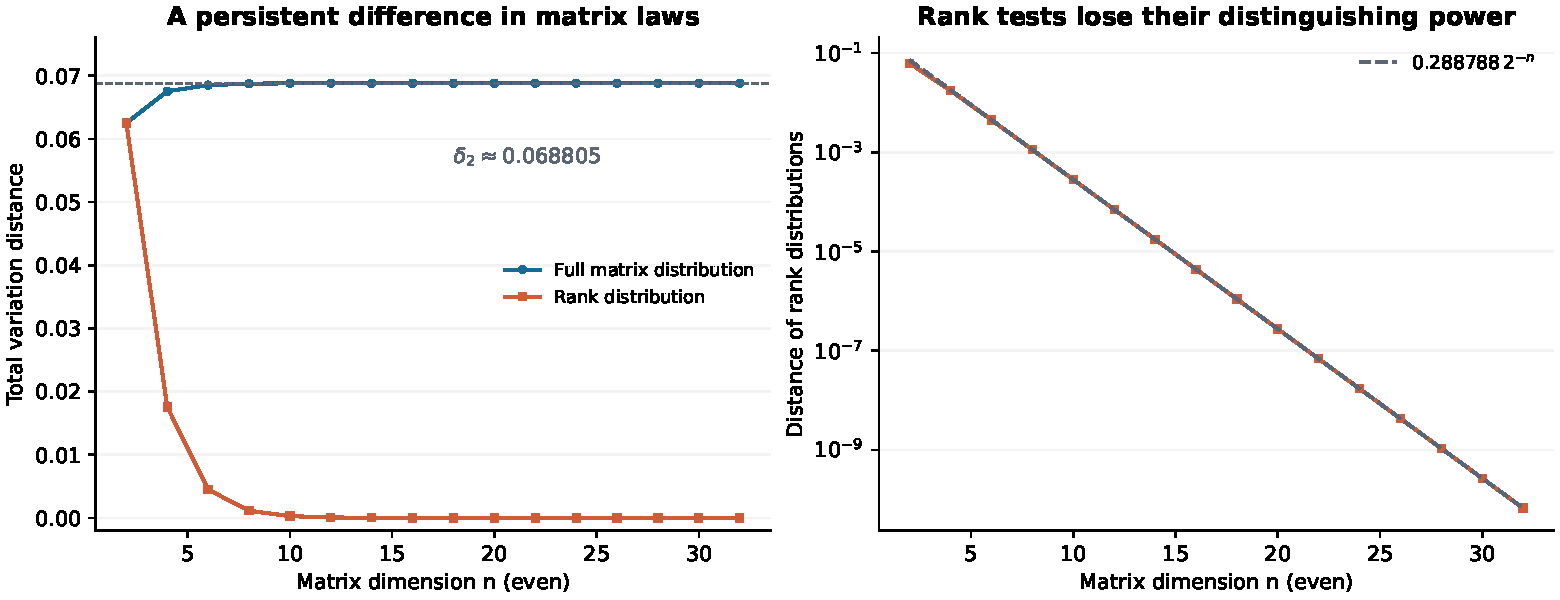
\includegraphics[width=\textwidth]{figures/rank_vs_matrix.pdf}
\caption{Exact rational formulas for $q=2$, displayed as real numbers. Left: full-matrix distance persists. Right: rank distance decays exponentially. No Monte Carlo sampling is used.}
\label{fig:main}
\end{figure}

\section{What the supplied sources contribute}
\subsection{Scope of the inspected Lean result}
We pinned \texttt{lsernau/grh-lean} at
\begin{center}\small\texttt{72fead102f663d5c7a407964a13dc0cf9d977207}.\end{center}
The declarations in \src{grh/src/Statements.lean}{\texttt{Statements.lean}} and exports in \src{grh/src/Main.lean}{\texttt{Main.lean}} state RH and GRH for every Dirichlet character of every modulus $N\ge1$. The half-plane statement excludes zeros for $\Re s>1/2$, with the principal-character point $s=1$ excepted. The strip statement places zeros with $0<\Re s<1$ on $\Re s=1/2$. These statements do not assert RH for arbitrary nonabelian Artin or automorphic $L$-functions \cite{repo}.

The repository reports checking with only the axioms \texttt{propext}, \texttt{Classical.choice}, and \texttt{Quot.sound}, as well as checks by additional kernel implementations. We inspected the public types, relevant proof files, configuration, and reported checks; we did not rebuild the complete development. The linked Wikipedia article reports the November 2026 proof and independent acceptance. We use that article as a map of the result and its context; the theorem types and reusable lemma come from primary source code \cite{wiki,repo}.

\subsection{The reusable mechanism}
The guide and reduction files compare upper and lower bounds on corrected lattice covolumes. Short integral forms, sufficient spanning by translates, and lower bounds for integral forms produce opposing estimates. Their main terms cancel in \src{grh/src/New/Reduction/MainInequality.lean}{\texttt{star\_inequality}}. The resulting one-sided weighted prime remainder is converted, using a polar Landau argument and a carefully chosen quadratic twist, into nonvanishing. The functional equation supplies the critical-line formulation \cite{reduction}.

The part used here is a finite-field second-moment argument from
\src{grh/src/New/Spanning/SecondMoment/PositiveType.lean}{\texttt{PositiveType.lean}}. In its notation, a nonnegative weight $\Theta$ on a finite group is of positive type when
$\Theta(a^{-1}b)=\langle u_a,u_b\rangle$ for vectors in a complex Hilbert space. For a representation $\pi:G\to\mathrm{GL}_N(\F)$ and two $N\times m$ matrices, a common stabilizer-mass bound $Y$ gives
\[
q\sum_{\det(A_1^{\mathsf T}\pi(g)A_0)=0}\Theta(g)
\le 2\sum_g\Theta(g)+q^{m+N/2}Y.
\]
Its Fourier estimate tensors character and delta vectors with $u_a$ and applies Cauchy--Schwarz. It makes compressed random matrices a natural direction in which to transfer the proof's methods \cite{positive}.

\subsection{Existing ProveIt results and the actual increment}
The ProveIt snapshot is
\begin{center}\small\texttt{9ce7302df13ca8ea547135be83c794141da8d79c}.\end{center}
We screened the READMEs of 61 research packets and the 103 text members of 29 newer incoming archives, then read the nearest finite-field predecessors. This is an overlap search, not a verification of every theorem in those packets. The directory itself records that the incoming research packets were filed as delivered and were not independently compiled or reviewed during placement \cite{proveit}.

The earlier rank-moment paper already gives a full hierarchy of kernel moments for positive-type weighted rectangular compressions. The earlier symplectic paper gives a general Fourier bound and computes the boundary law when the relevant source and target spaces are isotropic. In that case the conditional law given rank is uniform, so rank detects the entire distributional discrepancy. It explicitly asks for the effect of arbitrary restricted alternating forms \cite{moments,symprior}.

Our increment is the exact matrix likelihood for arbitrary input form with a Lagrangian projection, followed by a case where rank loses all asymptotic distinguishing power while the full law remains separated. This resolves the Lagrangian-output portion of that question. The problem with both compressed spaces arbitrary is not settled here.

Classical finite symplectic counts, Witt extension, and the uniform-matrix rank distribution are established tools. Relevant primary comparisons include Wan's and Guo--Li--Wang's counting work, Ishizuka's exact sampling paper, and Fulman--Goldstein's analysis of rank distributions \cite{wan,guo,ishizuka,fulman}. Targeted searches did not locate the precise likelihood and rank/full-law separation proved here. That supports a scoped novelty claim relative to the inspected material; it does not certify publication priority.

\section{Exact likelihood for every input alternating form}
The next theorem allows $H$ to be degenerate and $n$ to be odd. An alternating matrix has zero diagonal and satisfies $H^{\mathsf T}=-H$. The zero-diagonal requirement remains necessary in characteristic two.

Fix $n\ge1$, $0\le2s\le n$, and an alternating $H\in\Mat_n(\F)$ of rank $2s$. Put $d=n-2s$. Choose an injective $X_0$ with Gram matrix $H$, sample $g$ uniformly in $\Sp_{2n}(\F)$, and write $gX_0=(A;B)$. Such $X_0$ exists: embed a symplectic $2s$-space, then a $d$-dimensional isotropic subspace in its orthogonal complement.

For a fixed matrix $M$, let
\[
K=\ker M,\qquad k=\dim K,\qquad t=\dim(K\cap\rad H),\qquad
C_{n,s}=\prod_{j=s+1}^n(1-q^{-2j}).
\]
We call $K$ $H$-isotropic if $x^{\mathsf T}Hy=0$ for all $x,y\in K$.

\begin{theorem}[All-form projection likelihood]\label{thm:likelihood}
Relative to the uniform law on all $n\times n$ matrices,
\begin{equation}\label{eq:general-density}
\frac{\Pr(A=M)}{q^{-n^2}}=
\begin{cases}
\displaystyle\frac{q^{\binom{k}{2}}}{C_{n,s}}
\prod_{j=k-t+1}^{k}(1-q^{-j}),&K\text{ is }H\text{-isotropic},\\[6pt]
0,&\text{otherwise}.
\end{cases}
\end{equation}
Every product with no factors equals one. The formula is valid over every finite field, including those of characteristic two.
\end{theorem}

\subsection{Uniformity of the frame model and its normalization}
Witt extension says that an isometry between subspaces of a nondegenerate alternating space extends to an isometry of the whole space. Applied to the map between the columns of two injective frames with Gram matrix $H$, it shows that the group acts transitively on
\[
\mathcal X_H=\{X\in\Mat_{2n,n}(\F):\rank X=n,\ X^{\mathsf T}J_nX=H\}.
\]
Uniform $g$ therefore makes $gX_0$ uniform on $\mathcal X_H$; every point has the same number of preimages. This orbit principle is standard; see also the form-prescribed sampling framework in \cite{ishizuka}.

\begin{lemma}[Frame count]\label{lem:frames}
The number of frames in this orbit is
\begin{equation}\label{eq:frame-count}
|\mathcal X_H|=q^{n(3n+1)/2}C_{n,s}.
\end{equation}
\end{lemma}
\begin{proof}
A change of basis in the domain brings $H$ to a standard nondegenerate $2s$-block and a zero $d$-block. Choose the $s$ symplectic pairs of the first block in order. In a nondegenerate alternating space of dimension $2N$, the first member has $q^{2N}-1$ choices; its paired member with prescribed pairing one has $q^{2N-1}$ choices. Pass to their orthogonal complement after each pair. This gives
\[
\prod_{i=0}^{s-1}(q^{2n-2i}-1)q^{2n-2i-1}.
\]
The radical vectors must form an independent isotropic $d$-frame in the remaining nondegenerate space of dimension $2(n-s)$. After $i$ of them have been chosen, their orthogonal complement has dimension $2(n-s)-i$, and their own span has $q^i$ elements. The next vector thus has $q^{2(n-s)-i}-q^i$ choices. Multiply by
\[
\prod_{i=0}^{d-1}(q^{2(n-s)-i}-q^i).
\]
Extract powers of $q$. Their total exponent is $n(3n+1)/2$. The non-power factors in the first product have indices $n-s+1,\ldots,n$; those in the second have indices $s+1,\ldots,n-s$. Together they give $C_{n,s}$.
\end{proof}

\subsection{Counting the matrices below a specified projection}
\begin{lemma}[Fiber count]\label{lem:fiber}
For fixed $M$ with the notation of Theorem~\ref{thm:likelihood}, the number of $B$ such that $(M;B)\in\mathcal X_H$ is zero unless $K$ is $H$-isotropic. If it is isotropic, the number is
\begin{equation}\label{eq:fiber}
q^{n(n+1)/2+\binom{k}{2}}
\prod_{j=k-t+1}^{k}(1-q^{-j}).
\end{equation}
\end{lemma}
\begin{proof}
The Gram equation is
\begin{equation}\label{eq:gram}
M^{\mathsf T}B-B^{\mathsf T}M=H.
\end{equation}
Its restriction to $K\times K$ vanishes, proving necessity. Put $r=n-k$. Invertible matrices $P,T$ can bring $M$ to $PMT=\operatorname{diag}(I_r,0_k)$. Transform $B$ to $P^{-\mathsf T}BT$ and $H$ to $T^{\mathsf T}HT$ at the same time. These transformations preserve the equation, full rank of the frame, and the invariants $k,t$.

In these coordinates write
\[
M=\begin{pmatrix}I_r&0\\0&0\end{pmatrix},\quad
B=\begin{pmatrix}B_{11}&B_{12}\\B_{21}&B_{22}\end{pmatrix},\quad
H=\begin{pmatrix}H_{11}&H_{12}\\-H_{12}^{\mathsf T}&0\end{pmatrix}.
\]
Equation \eqref{eq:gram} becomes
\[
B_{11}-B_{11}^{\mathsf T}=H_{11},\qquad B_{12}=H_{12}.
\]
There are $q^{r(r+1)/2}$ choices for $B_{11}$: choose its diagonal and one entry from each off-diagonal pair freely. This argument works without division by two. There are $q^{kr}$ free choices for $B_{21}$.

On $K$, the kernel of $H_{12}$ is exactly $K\cap\rad H$, of dimension $t$. The whole frame is injective precisely when the map
$v\mapsto(H_{12}v,B_{22}v)$ on $K$ is injective. Equivalently, $B_{22}$ must be injective on the specified $t$-dimensional kernel of $H_{12}$. Its restriction to that space can be chosen in
\[
\prod_{i=0}^{t-1}(q^k-q^i)
\]
ways, with $q^{k(k-t)}$ extensions to $K$. This contributes
$q^{k^2}\prod_{j=k-t+1}^{k}(1-q^{-j})$. Finally,
\[
\frac{r(r+1)}2+kr+k^2=\frac{n(n+1)}2+\binom{k}{2},
\]
which proves the formula and sufficiency.
\end{proof}

Dividing \eqref{eq:fiber} by \eqref{eq:frame-count}, then by $q^{-n^2}$, proves Theorem~\ref{thm:likelihood}.

\begin{remark}[Why the nondegenerate endpoint simplifies]
If $H$ is nonsingular, $t=0$ for every $K$. Moreover, any solution of the Gram equation already makes $(M;B)$ injective: a vector in its kernel lies in $\rad H$. Thus the product correction disappears and every supported likelihood is strictly greater than one. If $H$ is degenerate, that last property can fail and must not be assumed.
\end{remark}

\section{Computing the complete law for arbitrary form rank}
The exact likelihood can be converted to finite sums with no enumeration of symplectic matrices.

Let $\gb{v}{j}$ denote the number of $j$-dimensional subspaces of $\F^v$; it is zero outside $0\le j\le v$. Let
\begin{equation}\label{eq:isocount}
I_s(l)=\prod_{i=0}^{l-1}\frac{q^{2s-i}-q^i}{q^l-q^i}
\quad(0\le l\le s),\qquad I_s(l)=0\text{ otherwise}.
\end{equation}
This is the number of isotropic $l$-subspaces in a nondegenerate alternating $2s$-space. Indeed, the numerator counts ordered independent isotropic vectors successively, and the denominator counts ordered bases of one $l$-space.

\begin{lemma}[Kernel types]\label{lem:types}
For $H$ of rank $2s$ and $d=n-2s$, the number of $H$-isotropic $k$-subspaces $K$ with $\dim(K\cap\rad H)=t$ is
\begin{equation}\label{eq:types}
N_{n,s}(k,t)=\gb{d}{t}\,q^{(d-t)(k-t)}I_s(k-t).
\end{equation}
An inadmissible index gives zero.
\end{lemma}
\begin{proof}
Choose $T=K\cap\rad H$ in $\gb{d}{t}$ ways. The image of $K$ in the nondegenerate quotient by $\rad H$ is an isotropic $(k-t)$-space, with $I_s(k-t)$ possibilities. After choosing a splitting of the quotient, $K/T$ is the graph of a linear map from that image to $\rad H/T$. There are $q^{(d-t)(k-t)}$ such maps. These choices are bijective with the required subspaces.
\end{proof}

For a uniform matrix, conditional on nullity $k$, its kernel is uniform among all $k$-subspaces: right multiplication by invertible matrices acts transitively on them. Therefore put
\[
w_{n,s}(k,t)=u_n(k)\frac{N_{n,s}(k,t)}{\gb{n}{k}},\qquad
L_{n,s}(k,t)=\frac{q^{\binom{k}{2}}}{C_{n,s}}
\prod_{j=k-t+1}^{k}(1-q^{-j}).
\]
The exact nullity probabilities and full distance are respectively
\begin{align}
\Pr(\dim\ker A=k)&=\sum_{t=0}^k w_{n,s}(k,t)L_{n,s}(k,t),\label{eq:all-ranklaw}\\
\TV(\Law(A),\Law(U_n))
&=1-\sum_{k=0}^n\sum_{t=0}^k
w_{n,s}(k,t)\min\{1,L_{n,s}(k,t)\}.\label{eq:all-fulltv}
\end{align}
The second identity follows by summing the overlap $\min(P(M),U(M))$ over every matrix. It automatically includes the mass of kernels that are not isotropic.

Formula \eqref{eq:uniform-nullity} itself follows by choosing the kernel, then choosing an injective map from its quotient into $\F^n$. This gives
\[
u_n(k)=q^{-n^2}\gb{n}{k}\prod_{i=0}^{n-k-1}(q^n-q^i),
\]
which simplifies to \eqref{eq:uniform-nullity}.

\begin{remark}[A characteristic-two detail]
For $q=2$, $k=t=2$, the numerator of the likelihood is
$2(1-2^{-1})(1-2^{-2})=3/4$. If $s\ge1$, then
$C_{n,s}>\prod_{j=2}^\infty(1-2^{-2j})>11/12$, so this supported likelihood is less than one. Consequently, for general degenerate $H$, full total variation is not just missing support. Formula \eqref{eq:all-fulltv} retains this case correctly.
\end{remark}

\begin{figure}[H]
\centering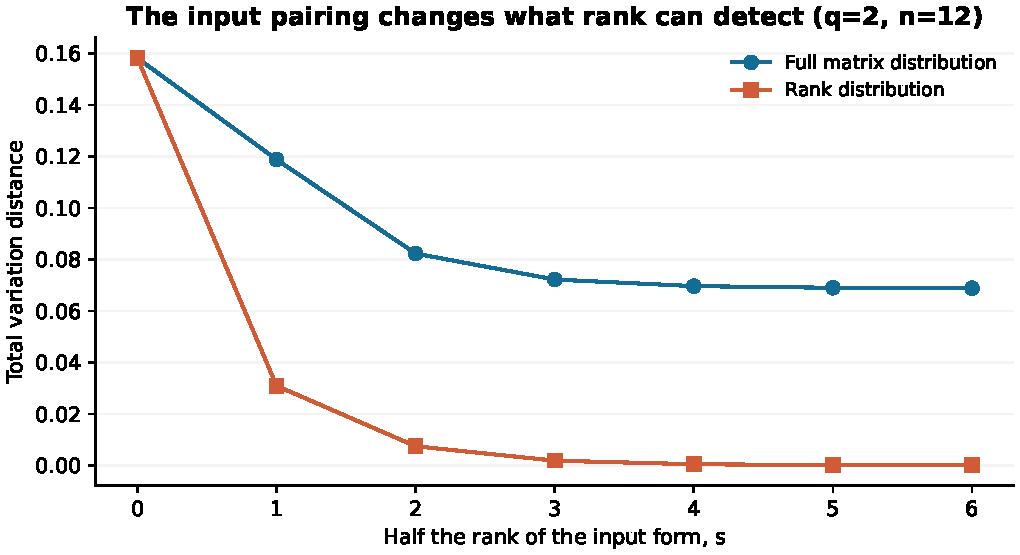
\includegraphics[width=.85\textwidth]{figures/form_type.pdf}
\caption{The all-form formulas at fixed $q=2,n=12$. At $s=0$ the input is isotropic; rank detects all discrepancy. At $s=6$ the input form is nonsingular; rank detects very little. Intermediate values come from the proved likelihood, without assuming monotonicity as a theorem.}
\end{figure}

\section{Exact separation when the input form is nondegenerate}
Assume $n=2m$ and $H$ is nonsingular. Theorem~\ref{thm:likelihood} becomes
\begin{equation}\label{eq:nondeg-density}
L(M)=\1_{\{\ker M\text{ is }H\text{-isotropic}\}}
\frac{q^{\binom{k}{2}}}{C_n}.
\end{equation}

\subsection{Nullity probabilities}
For $0\le k\le m$, define
\begin{equation}\label{eq:rnk-product}
R_{n,k}=\prod_{i=0}^{k-1}\frac{1-q^{2i-n}}{1-q^{i-n}},
\end{equation}
and set $R_{n,k}=0$ for $m<k\le n$. In particular $R_{n,0}=R_{n,1}=1$.
By dividing the isotropic ordered-frame count by the unrestricted ordered-frame count, the probability that a uniform $k$-subspace of $\F^n$ is $H$-isotropic is
\begin{equation}\label{eq:isoprob}
\alpha_{n,k}=q^{-\binom{k}{2}}R_{n,k}.
\end{equation}
Consequently \eqref{eq:nondeg-density} implies
\begin{equation}\label{eq:nondeg-ranklaw}
\Pr(\dim\ker A_n=k)=u_n(k)\frac{R_{n,k}}{C_n}.
\end{equation}

\begin{lemma}[All signs in the rank comparison]\label{lem:signs}
The ratio in \eqref{eq:nondeg-ranklaw} exceeds one for $k=0,1$ and is strictly less than one for every $k\ge2$.
\end{lemma}
\begin{proof}
The first assertion follows from $R_{n,0}=R_{n,1}=1>C_n$. If $k>m$, the ratio is zero. For $2\le k\le m$, each additional factor in \eqref{eq:rnk-product} is at most one, so
\[
R_{n,k}\le\frac{1-q^{2-n}}{1-q^{1-n}}.
\]
The deficit of this upper bound from one is
\[
\frac{(q^2-q)q^{-n}}{1-q^{1-n}}\ge q(q-1)q^{-n}.
\]
On the other hand, the elementary product bound $1-\prod(1-x_j)\le\sum x_j$ gives
\[
1-C_n\le\sum_{j=m+1}^n q^{-2j}<\frac{q^{-n}}{q^2-1}.
\]
Since $q(q-1)>1/(q^2-1)$, we have $R_{n,k}<C_n$. When $n=2$, the intermediate range is empty and the same conclusion follows directly.
\end{proof}

Total variation equals the sum of the positive discrepancies. By Lemma~\ref{lem:signs}, only nullities zero and one contribute. This proves \eqref{eq:rank-tv-main}. Using
\[
u_n(0)=a_n,\qquad
u_n(1)=a_n\frac{q}{(q-1)^2}(1-q^{-n})
\]
gives its second expression. The optimal rank-only event is exactly
$\{\dim\ker M\le1\}$, or equivalently $\{\rank M\ge n-1\}$.

\subsection{The full-matrix distance}
Since $0<C_n<1$ and $q^{\binom{k}{2}}\ge1$, \eqref{eq:nondeg-density} is greater than one at every supported matrix. All negative discrepancy from the uniform model is therefore on the complement of the support. Hence
\begin{equation}\label{eq:fullfinite}
\TV(\Law(A_n),\Law(U_n))
=1-\sum_{k=0}^n u_n(k)q^{-\binom{k}{2}}R_{n,k}.
\end{equation}
This proves the exact assertion and optimal event in \eqref{eq:full-tv-main}.

The mechanism is visible before counting: if $x,y\in\ker A_n$, then
\[
x^{\mathsf T}Hy
=x^{\mathsf T}(A_n^{\mathsf T}B_n-B_n^{\mathsf T}A_n)y=0.
\]
The nontrivial part of the theorem is that this obstruction remains statistically visible while the complete nullity distribution converges to the independent-entry law, with the exact exponential distance just proved.

\section{Limits and explicit constants}
\subsection{Asymptotics of the rank distance}
The infinite product $a_\infty$ is positive, since $\sum_{j\ge1}q^{-j}<\infty$. For fixed $q$,
\[
a_n=a_\infty(1+O_q(q^{-n})).
\]
Also
\[
\sum_{j=n/2+1}^{n}q^{-2j}
=\frac{q^{-n}(1-q^{-n})}{q^2-1}.
\]
The sum of terms containing at least two of these factors is $O_q(q^{-2n})$. Expanding the finite product and then its reciprocal gives
\[
C_n^{-1}-1=\frac{q^{-n}}{q^2-1}+O_q(q^{-2n}).
\]
Substitution into the exact rank distance proves \eqref{eq:rank-asymp-main}.

\subsection{The positive full-matrix limit}
For every fixed $k$,
\begin{equation}\label{eq:limiting-nullity}
u_n(k)\longrightarrow p_q(k):=a_\infty\frac{q^{-k^2}}{a_k^2},
\qquad R_{n,k}\longrightarrow1.
\end{equation}
One elementary way to justify passage to the infinite sum is to count kernel vectors. For a uniform matrix,
\begin{equation}\label{eq:uniform-firstmoment}
\E(q^{\dim\ker U_n})=1+(q^n-1)q^{-n}=2-q^{-n}<2.
\end{equation}
Thus the nullity tails are uniformly bounded by $2q^{-r}$ beyond $r$. Finite sums converge by \eqref{eq:limiting-nullity}; their tails tend uniformly to zero. Applying this to \eqref{eq:fullfinite} yields \eqref{eq:delta}. The $k=2$ term is positive, so $\delta_q>0$.

The classical limiting nullity law in \eqref{eq:limiting-nullity} also appears in \cite{fulman}; here the required convergence has been proved directly. No conjecture about zero ordinates or random-matrix models for zeta functions is involved.

\begin{center}
\begin{tabular}{rrr}
\toprule
$q$ & $\delta_q$ & coefficient of $q^{-n}$ in the rank distance\\
\midrule
2 & 0.0688050065066945 & 0.288788095086602\\
3 & 0.0132121494188950 & 0.122527579546740\\
4 & 0.00408561989901872 & 0.066303614685662\\
5 & 0.00165069311120747 & 0.041580699774208\\
\bottomrule
\end{tabular}
\end{center}

For $q=2$, exact finite formulas give:
\begin{center}
\begin{tabular}{rrr}
\toprule
matrix size $n$ & rank-law distance & full-matrix distance\\
\midrule
2  & $0.0625$ & $0.0625$\\
4  & $0.0175613702512$ & $0.0675354003906$\\
8  & $0.00112630708361$ & $0.0687307378366$\\
12 & $0.0000704980186387$ & $0.0688003837906$\\
16 & $0.00000440652973068$ & $0.0688047176613$\\
20 & $0.000000275409684107$ & $0.0688049884541$\\
\bottomrule
\end{tabular}
\end{center}

\subsection{A rigorous numerical enclosure}
The displayed limiting constants are not inferred from the finite tables. For integers $M\ge K$, the product tail satisfies
\[
a_M\left(1-\frac{q^{-M}}{q-1}\right)\le a_\infty\le a_M.
\]
Let $b_-$ be the positive lower bound on the left. For $k>K$,
$p_q(k)\le q^{-k^2}/a_\infty\le q^{-k^2}/b_-$. Hence the omitted part of \eqref{eq:delta} is at most
\begin{equation}\label{eq:certtail}
\frac{q^{-(K+1)^2}}{b_-(1-q^{-(2K+3)})}.
\end{equation}
Evaluating the finite sum with rational arithmetic, $M=140$, $K=12$, and outward-rounded decimal endpoints gives
\begin{gather*}
\delta_2>0.0688050065066945205731325149364250006122635,\\
\delta_2<0.0688050065066945205731325149364250006122636.
\end{gather*}
The rational interval before decimal rounding has width below $4.94\times10^{-44}$. The displayed decimal interval is wider because it is rounded outward. The script records both facts separately.

\section{Growing input-form rank: a broader version}
The separation is not confined to a nonsingular input form. The next theorem allows the radical dimension $n-2s$ to grow arbitrarily, as long as $s$ tends to infinity.

Write
\[
P_q=\prod_{j=1}^\infty(1-q^{-j}),\qquad
B_q=\prod_{j=1}^\infty(1-q^{-2j}),
\]
and set
\begin{equation}\label{eq:rateconstant}
\kappa_q=\frac1{2B_q}\left[
\frac1{q^2-1}+\frac1{P_q}
\left(\frac{2q+3}{q^2-1}+\frac{q}{(q-1)^2}\right)\right].
\end{equation}

\begin{theorem}[A growing symplectic part suffices]\label{thm:growing}
For the general form of rank $2s$ in Theorem~\ref{thm:likelihood},
\begin{equation}\label{eq:general-rate}
\TV(\Law(\dim\ker A),\Law(\dim\ker U_n))\le\kappa_q q^{-2s}.
\end{equation}
In particular $\kappa_2<12$. For every sequence with $s\to\infty$ and $2s\le n$, the full-matrix distance tends to the same constant $\delta_q$ in \eqref{eq:delta}.
\end{theorem}

\begin{proof}
Conditional on nullity $k$ in the uniform model, let $K$ be the uniform $k$-subspace. Put
\[
D_{n,k}=\prod_{i=0}^{k-1}(1-q^{i-n}),\qquad
F_{s,k}=\begin{cases}\prod_{i=0}^{k-1}(1-q^{2i-2s}),&k\le s,\\0,&k>s.\end{cases}
\]
Counting the $H$-isotropic $K$ with $K\cap\rad H=0$ by their image and graph in the quotient gives
\begin{equation}\label{eq:transverse-prob}
\Pr(K\text{ isotropic},\ t=0\mid k)
=q^{-\binom{k}{2}}\frac{F_{s,k}}{D_{n,k}}.
\end{equation}
For $k>s$ both sides are zero. Notice $D_{n,k}\ge P_q$.

Put $h(K)=\1_{\{K\text{ isotropic}\}}q^{\binom{k}{2}}
\prod_{j=k-t+1}^k(1-q^{-j})$. Then the rank likelihood is
$\E(h(K)\mid k)/C_{n,s}$. Its $t=0$ contribution is $F_{s,k}/D_{n,k}$, and its remaining contribution is between zero and
$q^{\binom{k}{2}}\Pr(t>0\mid k)$.

The expected number of lines of $K$ lying in the $d$-dimensional radical gives
\begin{align}
\Pr(t>0\mid k)
&\le\frac{(q^d-1)(q^k-1)}{(q-1)(q^n-1)}\nonumber\\
&\le\frac{q}{(q-1)^2}(q^k-1)q^{-2s}.\label{eq:radical-bound}
\end{align}
The product bound, extended by $F_{s,k}=0$ when $k>s$, gives
\begin{align}
\left|\frac{F_{s,k}}{D_{n,k}}-1\right|
&\le P_q^{-1}\left[q^{-2s}\frac{q^{2k}-1}{q^2-1}
 +q^{-n}\frac{q^k-1}{q-1}\right],\label{eq:product-bound}\\
1-C_{n,s}&\le\frac{q^{-2s}}{q^2-1},\qquad C_{n,s}\ge B_q.\nonumber
\end{align}
For $k>s$, the first numerator bound is still valid because
$q^{-2s}(q^{2k}-1)/(q^2-1)\ge1$.

Three uniform-model estimates finish the argument. The first is
$\E(q^k-1)\le1$ from \eqref{eq:uniform-firstmoment}. Counting pairs of kernel vectors according to whether they span a space of dimension zero, one, or two gives
\[
\E q^{2k}=1+(q+1)(1-q^{-n})
 +(1-q^{-n})(1-q^{1-n})\le q+3.
\]
Finally \eqref{eq:uniform-nullity} implies the useful majorant
\[
u_n(k)\le P_q^{-1}q^{-k^2}.
\]
Indeed $a_n\le a_k,a_{n-k}$. Therefore
\begin{align*}
\E\bigl[q^{\binom{k}{2}}(q^k-1)\bigr]
&\le P_q^{-1}\sum_{k\ge1}
\left(q^{-k(k-1)/2}-q^{-k(k+1)/2}\right)\\
&=P_q^{-1}.
\end{align*}
Using $q^{-n}\le q^{-2s}$, sum \eqref{eq:radical-bound} and \eqref{eq:product-bound} against $u_n(k)$, divide by $2C_{n,s}$, and include the normalization error $1-C_{n,s}$. The result is exactly \eqref{eq:general-rate} with \eqref{eq:rateconstant}.

For the full-law limit, work again conditional on $k$. On the event in \eqref{eq:transverse-prob}, the matrix likelihood is $q^{\binom{k}{2}}/C_{n,s}\ge1$. Off the isotropic event it is zero. Contributions with $t>0$ have total uniform probability tending to zero by \eqref{eq:radical-bound}. For fixed $k$, \eqref{eq:transverse-prob} tends to $q^{-\binom{k}{2}}$ as $s\to\infty$. Thus the conditional negative discrepancy tends to $1-q^{-\binom{k}{2}}$. The uniform nullity tail bound \eqref{eq:uniform-firstmoment} permits summation over $k$, giving $\delta_q$.
\end{proof}

The assertion $\kappa_2<12$ can be checked with the same product-tail enclosure used for $\delta_2$; rough bounds $P_2>0.2887$ and $B_2>0.6885$ already suffice in \eqref{eq:rateconstant}. This rate is not claimed sharp for all degeneracies. The nondegenerate formula is sharper and exact.

\section{Verification, formalization, and limits of the claim}
\subsection{Computational verification}
The archive contains two independent styles of check.
\begin{enumerate}
\item \texttt{code/exhaustive\_check.py} enumerates actual pairs $(A,B)$ over prime fields, computes full rank and the actual Gram matrix, and compares the resulting fiber counts with Lemma~\ref{lem:fiber}. The cases $(q,n)=(2,2),(3,2),(2,3)$ cover 268,961 pairs and 4,371 individual $(A,H)$ comparisons. All pass. The larger case covers several degenerate forms in characteristic two.
\item \texttt{code/verify\_formulas.py} uses integers and rational numbers to evaluate the general laws. It verifies normalization, a first kernel moment, data processing, the exact nondegenerate distances, and all rank-comparison signs in 288 parameter cases: $q\in\{2,3,4,5,8,9\}$, $1\le n\le12$, $0\le s\le\lfloor n/2\rfloor$. Extension-field cases here test the prime-power counting formulas, not a field-arithmetic implementation.
\end{enumerate}
All reported finite tables are exact rational evaluations followed by decimal display. The figures use those formulas. The infinite constants have explicit rational enclosures from \eqref{eq:certtail}. None of these checks is substituted for a proof over arbitrary $q,n$.

\subsection{Formalization boundary}
The new theorem has not been compiled in Lean. The archive's formalization plan specifies finite sets of frames, the block-equation bijections, the kernel-type count, rational probability masses, and the finite total-variation identities as separate obligations. The infinite-product and limit arguments form a later analytic layer. No placeholder is presented as a completed proof.

The upstream proof is a separate artifact: its reported kernel checks and its exported propositions do not by themselves certify this new theorem. Conversely, our finite-field proof does not require importing the large GRH development. The source lemma motivates the research direction; the final proof uses direct counting.

\subsection{What has and has not been resolved}
We have determined the law for a Lagrangian projection of an arbitrary $n$-dimensional input subspace, including its full alternating form and radical. We have proved an exact finite-dimensional separation between rank tests and full matrix tests at the nondegenerate endpoint, and a broader separation when the input-form rank grows. The remaining classification with both compressed spaces arbitrary requires further work.

The contribution is a new result derived in this investigation and absent from the inspected ProveIt predecessors. We do not claim that standard symplectic counts are new, that a major named conjecture beyond the supplied RH/Dirichlet-GRH result has been resolved, or that literature priority has been exhaustively established.

\appendix
\section{Reproduction and source provenance}
From the extracted archive directory:
\begin{verbatim}
python3 code/verify_formulas.py
python3 code/exhaustive_check.py
python3 code/make_figures.py
latexmk -pdf -interaction=nonstopmode -halt-on-error paper.tex
\end{verbatim}
The first two scripts use only the Python standard library. Plotting additionally needs Matplotlib. The TeX source uses standard LaTeX packages. \texttt{results/} contains the saved check outputs, exact finite-distance tables, and certified constant intervals. \texttt{provenance/} contains the pinned audit and selected source files with their original notices. A SHA-256 manifest records the delivered contents.

The upstream source was read at a fixed commit; copied files were checked against Git blob hashes. The ProveIt catalogue records the screened packets and archive members. This note introduces no remote repository change.

\begin{thebibliography}{99}\small\raggedright
\bibitem{repo} L. Sernau and collaborators, after L. Alp\"oge with Claude.
\emph{GRH for Dirichlet $L$-functions, in Lean 4}.
\href{https://github.com/lsernau/grh-lean}{Repository}, commit
\texttt{72fead102f663d5c7a407964a13dc0cf9d977207}, inspected 26 November 2026.
See \src{grh/src/Statements.lean}{public statements}, \src{grh/src/Main.lean}{exports}, and \src{grh/README.md}{reported checks}.
\bibitem{reduction} Same repository.
\src{grh/GUIDE.md}{\texttt{grh/GUIDE.md}};
\src{grh/src/New/Reduction/MainInequality.lean}{\texttt{MainInequality.lean}};
\src{grh/src/New/Reduction/OneSidedBound.lean}{\texttt{OneSidedBound.lean}};
\src{grh/src/New/Reduction/Zeros/Criterion.lean}{\texttt{Zeros/Criterion.lean}};
\src{grh/src/New/Reduction/Zeros/PrimeError.lean}{\texttt{Zeros/PrimeError.lean}}.
\bibitem{positive} Same repository.
\src{grh/src/New/Spanning/SecondMoment/PositiveType.lean}{\emph{Functions of positive type and singular minors}}, especially
\texttt{re\_sum\_addChar\_dotProduct\_mul\_le} and
\texttt{card\_mul\_sum\_det\_eq\_zero\_le}.
\bibitem{proveit} V. Reshetnikov, \emph{ProveIt: Analysis/GeneralizedRiemannHypothesis},
\href{https://github.com/VladimirReshetnikov/ProveIt/tree/main/Analysis/GeneralizedRiemannHypothesis}{repository directory}, commit
\texttt{9ce7302df13ca8ea547135be83c794141da8d79c}.
\bibitem{moments} ProveIt research packet,
\prior{Research/grh_beyond_dirichlet_2026-11-25/sections/rank_moments.tex}{\emph{Rank moments}}, 25 November 2026.
\bibitem{symprior} ProveIt research packet,
\prior{Research/grh_sharp_torsion_and_symplectic_blocks/report.tex}{\emph{Beyond Dirichlet GRH: sharp specialization and random symplectic blocks}}, especially
\prior{Research/grh_sharp_torsion_and_symplectic_blocks/symplectic.tex}{the symplectic-block section} and its final questions.
\bibitem{wiki} Wikipedia contributors, \emph{Riemann hypothesis},
\url{https://en.wikipedia.org/wiki/Riemann_hypothesis}, accessed 26 November 2026. Used for current context; proof inputs are sourced separately.
\bibitem{wan} Z.-X. Wan, \emph{Anzahl theorems in finite singular symplectic, unitary and orthogonal geometries}, Discrete Mathematics (1993),
\href{https://doi.org/10.1016/0012-365X(93)90013-J}{doi:10.1016/0012-365X(93)90013-J}.
\bibitem{guo} J. Guo, F. Li, K. Wang,
\emph{Anzahl formulas of subspaces in symplectic spaces and their applications},
Linear Algebra and its Applications \textbf{438} (2013), 3321--3335,
\href{https://doi.org/10.1016/j.laa.2012.12.008}{doi:10.1016/j.laa.2012.12.008}.
\bibitem{ishizuka} K. Ishizuka,
\emph{Uniform Sampling of Linear Codes with Prescribed Hull Dimension},
\href{https://arxiv.org/html/2611.03578v2}{arXiv:2611.03578v2}, 25 November 2026, especially Sections 3.2 and 4. The symplectic mass formula is attributed there to classical finite-geometry work.
\bibitem{fulman} J. Fulman and L. Goldstein,
\emph{Stein's method and the rank distribution of random matrices over finite fields},
Annals of Probability \textbf{43} (2015), 1274--1314,
\href{https://arxiv.org/abs/1211.0504}{arXiv:1211.0504};
\href{https://doi.org/10.1214/13-AOP889}{doi:10.1214/13-AOP889}.
\end{thebibliography}
\end{document}
